\section{Auswertung}
\subsection{{\texorpdfstring{$\gamma$}{Gamma}}- Strahlung}
\subsubsection{Nulleffekt}
Ohne Strahler werden durch Hintergrundsstrahlung bedingt $N = 1229$ Impulse in $t_0 = 1000\,\symup{s}$ aufgenommen. Dadurch ergibt sich eine Zählrate von

\begin{equation}
Z_{\text{u}} = \frac{N_{\text{u}}}{t} = \frac{1229}{1000\,\symup{s}} = 1{,}23\,\frac{1}{\symup{s}}.
\label{eqn:zaehlrate}
\end{equation}
Der Fehler der Zählrate lässt sich über

\begin{equation}
\sigma_{\text{Z}} = \frac{\sqrt{N}}{t}
\label{eqn:fehlerzaehlrate}
\end{equation}
berechnen. Damit ergibt sich der fehlerbehaftete Wert der Zählrate von 

\begin{equation*}
Z_{\text{u}} =  (1{,}23 \pm 0{,}04)\,\frac{1}{\symup{s}}.
\end{equation*}







\subsubsection{Experimentell}
In den Tabellen \ref{tab:blei} und \ref{tab:eisen} sind die aufgenommenen Werte der Untersuchungen von Blei- und Eisenabsorber, sowie auch weitere, daraus errechneten Werte zu finden. Hierbei ist $d$ die Dicke des Absorbers, $t$ die Messzeit, $N$ die Anzahl
der Impulse und $\sigma_{\text{N}}$ der dazugehörige Fehler, welcher der Wurzel von $N$ entspricht. $Z$ ist die Zählrate mit dem Fehler $\sigma_{\text{Z}}$, welche mit \ref{eqn:zaehlrate} und \ref{eqn:fehlerzaehlrate} berechnet werden, $(Z - Z_{\text{u}})$
ist die Differenz der Zählrate und dem Nulleffekt, die mit $\symup{ln}(Z - Z_{\text{u}})$ zudem logarithmiert wird. Der Fehler des letzten Wertes wird mit

\begin{equation*}
\sigma_{\text{Z - Zu}} = \sqrt{\biggl(\frac{\sqrt{N}}{t}\biggr)^2 + \biggl(\frac{\sqrt{N_{\text{u}}}}{t_0}\biggr)^2}
\end{equation*}
berechnet.


\begin{table}[htbp]
\centering
\caption{Messwerte Blei. }
\label{tab:blei}
\begin{tabular}{S[table-auto-round, table-format=1.2] S[table-auto-round, table-format=3] S[table-auto-round, table-format=4] S[table-auto-round, table-format=2.1] S S[table-auto-round, table-format=3.1] S[table-auto-round, table-format=1.1] S[table-auto-round, table-format=3.1] S[table-auto-round, table-format=1.1] S}
\toprule
{$d/10^{-2} \, \symup{m}$} & {$t/ \, \symup{s}$} & {$N$} & {$\sigma_{\text{N}}$} & {$Z/\,\symup{\frac{1}{s}}$} & {$\sigma_{\text{Z}}$} & {$(Z - Z_{\text{u}})$} & {$\symup{ln}(Z - Z_{\text{u}})$} & {$\sigma_{\text{Z - Zu}}$}\\
\midrule
0.12 & 50 & 6975 & 83.5 & 139.5 & 1.7 & 138.3 & 4.9 & 1.7\\
1    & 100 & 4976 & 70.5 & 49.8 & 0.7 & 48.6 & 3.88 & 0.7\\
1.12 & 150 & 6776 & 82.3 & 45.2 & 0.5 & 43.9 & 3.8 & 0.6\\
2    & 200 & 3693 & 60.7 & 18.5 & 0.3 & 17.3 & 2.9 & 0.3\\
2.12 & 250 & 4402 & 66.3 & 17.6 & 0.3 & 16.4 & 2.8 & 0.3 \\
3    & 300 & 2107 & 45.9 & 7.0 & 0.2 & 5.8 & 1.8 & 0.2 \\
3.12 & 350 & 2410 & 49.1 & 6.9 & 0.1 & 5.7 & 1.7 & 0.1 \\
6    & 400 & 1220 & 34.9 & 3.1 & 0.1 & 1.9 & 0.6 & 0.1\\
\bottomrule
\end{tabular}
\end{table}

\begin{table}[htbp]
\centering
\caption{Messwerte Eisen. }
\label{tab:eisen}
\begin{tabular}{S[table-auto-round, table-format=1.2] S[table-auto-round, table-format=3] S[table-auto-round, table-format=4] S[table-auto-round, table-format=2.1] S S[table-auto-round, table-format=3.1] S[table-auto-round, table-format=1.1] S[table-auto-round, table-format=3.1] S[table-auto-round, table-format=1.1] S}
\toprule
{$d/10^{-2} \, \symup{m}$} & {$t/ \, \symup{s}$} & {$N$} & {$\sigma_{\text{N}}$} & {$Z/\,\symup{\frac{1}{s}}$} & {$\sigma_{\text{Z}}$} & {$(Z - Z_{\text{u}})$} & {$\symup{ln}(Z - Z_{\text{u}})$} & {$\sigma_{\text{Z - Zu}}$}\\
\midrule
0.5  & 50 & 5760 & 75.9 & 115.2 & 1.5 & 113.9 & 4.7 & 1.5\\
1    & 60 & 5396 & 73.5 & 89.9 & 1.2 & 88.7 & 4.5 & 1.2\\
1.5  & 94 & 6712 & 81.9 & 71.4 & 0.9 & 70.2 & 4.3 & 0.9 \\
2    & 75 & 4460 & 66.8 & 59.5 & 0.9 & 58.3 & 4.1 & 0.9\\
2.5  & 125 & 5512 & 74.2 & 44.1 & 0.6 & 42.9 & 3.8 & 0.6\\
3    & 135 & 4605 & 67.9 & 34.1 & 0.5 & 32.9 & 3.5 & 0.5\\
3.5  & 145 & 3956 & 62.9 & 27.3 & 0.4 & 26.1 & 3.3 & 0.4 \\
6    & 155 & 3578 & 59.8 & 23.1 & 0.4 & 21.9 & 3.1 & 0.4 \\
\bottomrule
\end{tabular}
\end{table}

Werden nun die Werte von $\symup{ln}(Z - Z_{\text{u}})$ gegen die Dicke $d$ aufgetragen und mithilfe von Scipy curve-fit eine lineare Ausgleichsrechnung vorgenommen, so ergeben sich die in Abbildung \ref{fig:ausgleichsgerade} zu sehenden Geraden.

\begin{figure}[h!tbp]
	\centering
	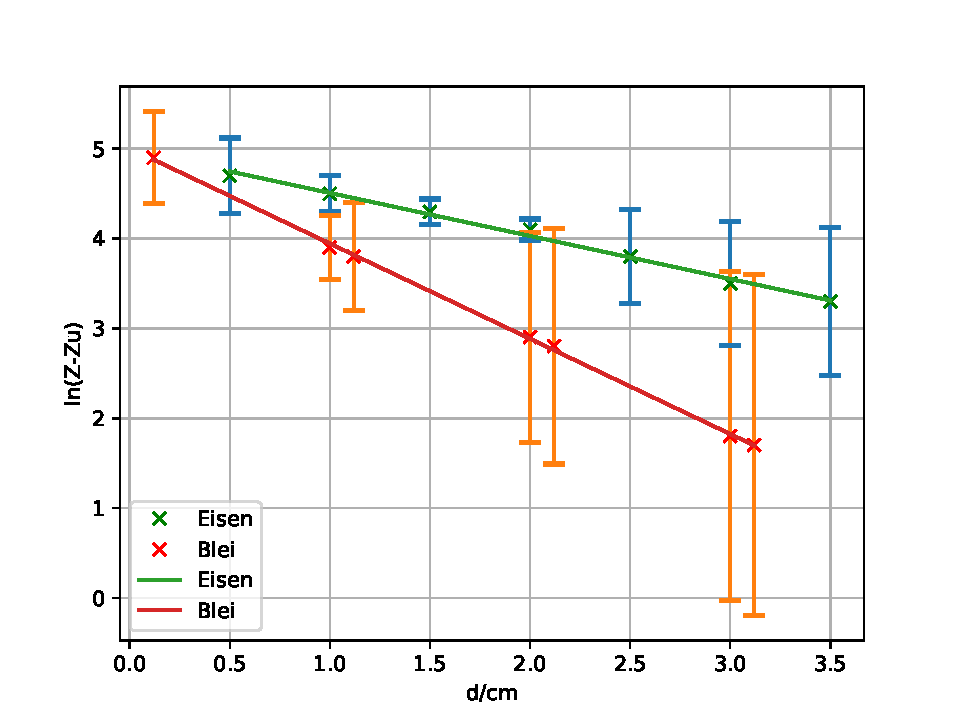
\includegraphics[width=0.8\linewidth]{Graphik1.pdf}
	\caption{Ausgleichsrechnung für Blei- und Eisenabschirmung.}
	\label{fig:ausgleichsgerade}
\end{figure}
Die Geraden haben nach dem Absorptionsgesetz \ref{eq:eq1} die Form

\begin{equation*}
\symup{ln}(Z_{\text{D}}) = \symup{ln}(Z_0) + \mu d.
\end{equation*}
Somit ist $\symup{ln}(Z_0)$ der Y-Achsenabschnitt und $\mu$ die Absorptionskonstante.
Die Ausgleichsrechnung liefert die folgenden Werte der beiden Geraden:

\begin{equation*}
\begin{aligned}
\text{Blei:}\,\, &\mu_{\text{Blei}} = (105{,}998 \pm 0{,}015)\,\symup{\frac{1}{m}} \\
      &\symup{ln}_{\text{Blei}} = (5{,}0041 \pm 0{,}0006) \\
\text{Eisen:}\,\, &\mu_{\text{Eisen}} = (47{,}86 \pm 0{,}03)\,\symup{\frac{1}{m}} \\
      &\symup{ln}_{\text{Eisen}} = (4{,}9857 \pm 0{,}0015)\\
\end{aligned}
\end{equation*}






\subsubsection{Theoretisch}
Die theoretischen Werte der Absorptionskoeffizienten $\mu_{\text{com}}$ werden über Gleichung \ref{eq:absorptionskoeffizient} berechnet. Der dafür benötigte Wirkungsquerschnitt ergibt sich aus Gleichung \ref{eq:wirkungsquerschnitt}, wobei für 
den Elektronenradius $r_{\text{e}} = 2{,}8\cdot10^{-15}\,\symup{m}$ eingesetzt wird. Der Wert für $\epsilon$ für Cäsium-137 wird aus der Versuchsanleitung entnommen und beträgt $\epsilon = 1{,}295$ \cite[14]{anleitung704}. Die Ordnungszahlen $Z$,
Dichten $\rho$ und molaren Massen $M$ sind in Tabelle \ref{tab:litwerte} zu finden.

\begin{table}[htbp]
\centering
\caption{Literaturwerte für Blei und Eisen.\cite{blei} \cite{eisen}}
\label{tab:litwerte}
\begin{tabular}{S S[table-auto-round, table-format=2] S[table-auto-round, table-format=3.3] S[table-auto-round, table-format=5] }
\toprule
& {$Z$} & {$M/10^{-3}\,\symup{\frac{kg}{mol}}$} & {$\rho/\,\symup{\frac{kg}{m^3}}$}\\
\midrule
$\text{Blei}$  & 82 & 207.2 & 11340 \\
$\text{Eisen}$ & 26 & 55.845 & 7874 \\

\bottomrule
\end{tabular}
\end{table}
Werden die entsprechenden Werte in \ref{eq:absorptionskoeffizient} eingesetzt, so ergeben sich für die theoretischen Absorptionskoeffizienten von Blei und Eisen:

\begin{equation*}
\begin{aligned}
\mu_{\text{com,Blei}} &= 69{,}19 \,\symup{\frac{1}{m}} \\
\mu_{\text{com,Eisen}} &= 56{,}5 \,\symup{\frac{1}{m}} \\
\end{aligned}
\end{equation*}









\subsection{{\texorpdfstring{$\beta$}{Beta}}-Strahlung}
Ohne den $\beta$-Strahler werden $N = 614$ Impulse in $t_0 = 1000\,\symup{s}$ aufgenommen. Damit ist die Zählrate:

\begin{equation}
Z_{\text{u}} = \frac{N_{\text{u}}}{t} = \frac{614}{1000\,\symup{s}} = 0{,}61\,\frac{1}{\symup{s}}.
\label{eqn:zaehlrate}
\end{equation}
Der Fehler der Zählrate wird über \ref{eqn:fehlerzaehlrate} berechnet. Es ergibt sich der fehlerbehaftete Wert der Zählrate von 
\begin{equation*}
Z_{\text{u}} =  (0{,}61 \pm 0{,}02)\,\frac{1}{\symup{s}}.
\end{equation*}


\subsubsection{Experimentell}
Die Berechnung der einzelnen Werte erfolgt analog zu denen für Blei und Eisen. Zusätzlich ist in Tabelle \ref{tab:aluminium} die Massenbelegung $R$ aufgeführt, die mit

\begin{equation*}
R = \rho \cdot d
\end{equation*}
bestimmt wird. Dabei ist die Dichte für Aluminium $\rho = 2700\,\symup{\frac{kg}{m^3}}$.

\begin{table}[htbp]
\centering
\caption{Messwerte Aluminium. }
\label{tab:aluminium}
\begin{tabular}{S[table-auto-round, table-format=3] S[table-auto-round, table-format=1.2] S[table-auto-round, table-format=3] S[table-auto-round, table-format=4] S[table-auto-round, table-format=2.1] S S[table-auto-round, table-format=3.1] S[table-auto-round, table-format=1.1] S[table-auto-round, table-format=3.1] S[table-auto-round, table-format=1.2] S}
\toprule
{$d/10^{-6} \, \symup{m}$} & {$R/\,\symup{\frac{g}{cm^2}}$} &{$t/ \, \symup{s}$} & {$N$} & {$\sigma_{\text{N}}$} & {$Z/\,\symup{\frac{1}{s}}$} & {$\sigma_{\text{Z}}$} & {$(Z - Z_{\text{u}})$} & {$\symup{ln}(Z - Z_{\text{u}})$} & {$\sigma_{\text{Z - Zu}}$}\\
\midrule
0   & 0   & 60 & 34112 & 184.7 & 568.5 & 3.08 & 567.9 & 6.3 & 3.08\\
100 & 0.03 & 60 & 2412  & 49.1  & 40.2  & 0.82 & 39.6 &  3.7 & 0.82\\
125 & 0.03 & 60 & 608   & 24.7  & 10.1  & 0.41 &  9.5 &  2.3 & 0.41\\
153 & 0.04 & 60 & 543   & 23.3  & 9.1   & 0.39 &  8.5 &  2.1 & 0.39\\
160 & 0.04 & 80 & 422   & 20.5  & 5.3   & 0.26 &  4.7 &  1.5 & 0.26\\
200 & 0.05 & 150 & 317  & 17.8  & 2.1   & 0.12 &  1.5 &  0.4 & 0.12\\
253 & 0.07 & 350 & 287  & 16.9  & 0.8   & 0.05 &  0.2 & -1.6 & 0.05 \\
302 & 0.08 & 600 & 442  & 21.0  & 0.7   & 0.04 &  0.1 & -2.3 & 0.04 \\
338 & 0.09 & 600 & 411  & 20.3  & 0.7   & 0.03 &  0.1 & -2.3 & 0.04 \\
400 & 0.11 & 600 & 416  & 20.4  & 0.7   & 0.03 &  0.1 & -2.3 & 0.04 \\
444 & 0.12 & 600 & 424  & 20.6  & 0.7   & 0.03 &  0.1 & -2.3 & 0.04 \\
482 & 0.13 & 700 & 489  & 22.1  & 0.7   & 0.03 &  0.1 & -2.3 & 0.04 \\
\bottomrule
\end{tabular}
\end{table}
Nun wird $\symup{ln}(Z - Z_{\text{u}})$ gegen die Massenbelegung $R$ aufgetragen. Es gibt sich die in Abbildung \ref{fig:aluminium} zu sehende Kurve.

\begin{figure}[h!tbp]
	\centering
	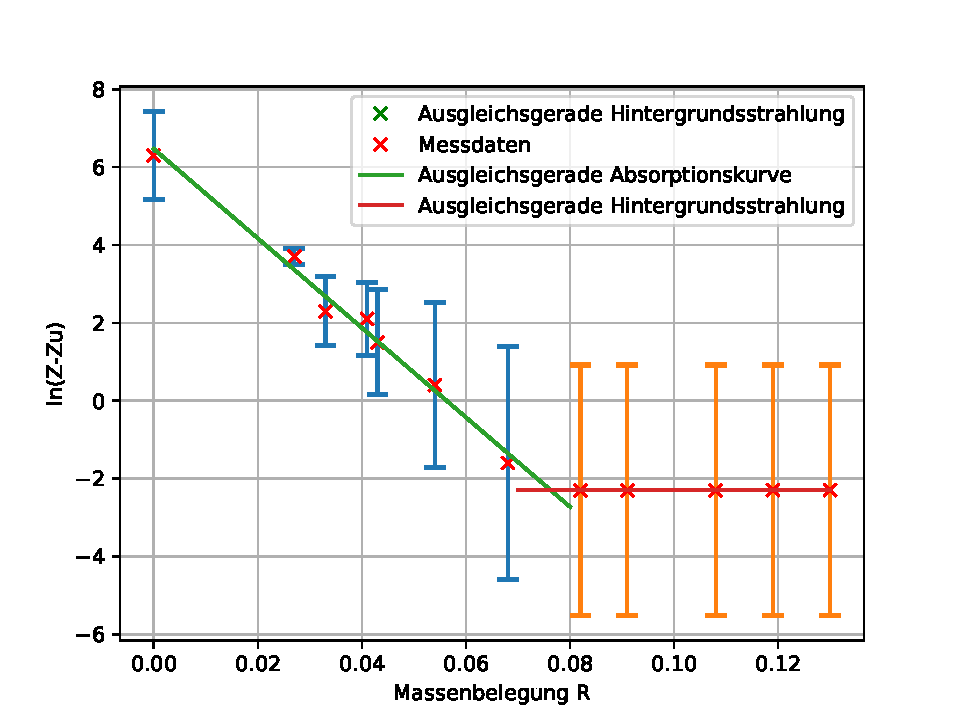
\includegraphics[width=0.8\linewidth]{alu.pdf}
	\caption{Ausgleichsrechnung für Aluminiumabschirmung.}
	\label{fig:aluminium}
\end{figure}
Durch diese wird mit Scipy curve-fit eine Ausgleichsgerade für die Absorptionskurve und eine für die Hintergrundsstrahlung gelegt.
Für die Ausgleichsgerade der Absorptionkurve der Form $y = ax + b$ werden die Werte

\begin{equation*}
\begin{aligned}
a &= (-114{,}9 \pm 34{,}8)\,\symup{\frac{m^2}{kg}} \\
b &= 6{,}47 \pm 0{,}06
\end{aligned}
\end{equation*}
ausgegeben, die Parameter für die lineare Regression der Hintergrundsstrahlung mit $y = ex + f$ sind

\begin{equation*}
\begin{aligned}
e &= (-8{,}9\cdot10^{-8} \pm 2{,}9\cdot10^{-17})\,\symup{\frac{m^2}{kg}} \\
f &= -2{,}3 \pm 1{,}4\cdot10^{-18}
\end{aligned}
\end{equation*}
Zur Bestimmung der maximalen Reichweite $R_{\text{max}}$ werden die Geradengleichungen gleichgesetzt und umgestellt:

\begin{equation}
x = R_{\text{max}} = \frac{f - b}{a - e}
\label{eq:reichweite}
\end{equation}
Da alle Parameter fehlerbehaftet sind, muss der Fehler $\sigma_{\text{R,max}}$ mit der Gaußschen Fehlerfortpflanzung berechnet werden:

\begin{equation}
\begin{aligned}
\Delta_{\text{R,max}} &= \sqrt{\biggl(\frac{\partial x}{\partial a}\biggr)^2 \Delta a^2 + \biggl(\frac{\partial x}{\partial b}\biggr)^2 \Delta b^2 + \biggl(\frac{\partial x}{\partial e}\biggr)^2 \Delta e^2 + \biggl(\frac{\partial x}{\partial f}\biggr)^2 \Delta f^2} \\
                      &= \sqrt{\biggl(\frac{b-f}{(a-e)^2}\biggr)^2 \Delta a^2 + \biggl(-\frac{1}{a-e}\biggr)^2 \Delta b^2 + \biggl(\frac{f - b}{(a - e)^2}\biggr)^2 \Delta e^2 + \biggl(\frac{1}{a - e}\biggr)^2 \Delta f^2} \\
\label{eq:reichweitefehler}
\end{aligned}
\end{equation}
Werden alle Parameter in \ref{eq:reichweite} und \ref{eq:reichweitefehler} eingesetzt, so ergibt sich eine maximale Reichweite von

\begin{equation*}
R_{\text{max}} = (0{,}076 \pm 0{,}02)\,\symup{\frac{g}{cm^2}}.
\end{equation*}
Zur Bestimmung der Gesamtenergie $E_{\text{max}}$ wird Formel \ref{eq:gesamtenergie} verwendet. Auch hier muss der Fehler berücksichtigt werden:

\begin{equation*}
\Delta E_{\text{max}} = \sqrt{\Biggl(\frac{1{,}92(2R_{\text{max}}^2+0{,}22)}{2\sqrt{R_{\text{max}}^2+0{,}22R_{\text{max}}}}\Biggr)^2 \Delta R_{\text{max}}^2 }
\end{equation*}
Die maximale Gesamtenergie ist damit

\begin{equation*}
E_{\text{max}} = (0{,}29 \pm 0{,}03)\,\symup{MeV}.
\end{equation*}